\documentclass[aps,prd,onecolumn,superscriptaddress,showpacs,12pt]{revtex4-2}

\usepackage{lmodern}
\usepackage[T1]{fontenc}
\usepackage{amsmath,amssymb,amsthm}
\usepackage{graphicx}
\usepackage{booktabs}
\usepackage{hyperref}
\usepackage{bm}

\newcommand{\taudeath}{\tau_{\mathrm{death}}}
\newcommand{\chic}{\chi_c}
\newcommand{\sigmad}{\sigma_d}
\newcommand{\Rzero}{R_0}
\newcommand{\Iphase}{I_{\mathrm{phase}}}
\newcommand{\writeback}{s_h(i)}
\newcommand{\meancoupling}{\bar{c}_h}

\newtheorem{proposition}{Proposition}[section]
\newtheorem{remark}{Remark}[section]

\begin{document}

\title{Coherence-Guided Dead-Head Identification in Frozen Transformers:\\
A Zero-Parameter Geometric Threshold from Coupled-Oscillator Criticality}

\author{Michael Sharpe}
\affiliation{Project 89 / Green Loom Association}

\date{March 2026}

\begin{abstract}
We test a narrow hypothesis: dead attention heads in a frozen transformer obey a
coherence boundary that can be derived from coupled-oscillator criticality rather
than fitted from model-specific calibration. The claim of this paper is an
identification law, not a complete removal procedure. The operational observable is
head-level coupling between a head's incoming attention-weighted value write-back
and the receiver's pre-head residual stream. The geometric interpretation is
explicit: LayerNorm places token states approximately on $S^{d-1}$, attention
heads act as state-dependent inter-oscillator couplings, and MLP updates act as
intra-oscillator modes. Starting from the lattice Coherence Learning Rule (CLR)
bond-death threshold $\cos(\Delta \theta) = 0.679$ on $S^1$, normalizing by the
natural fluctuation scale on the circle, and then rescaling by concentration of
measure on $S^{d-1}$ yields a transformer death threshold
\begin{equation}
\boxed{\taudeath(d) = \frac{\chic}{\sqrt{d}}}, \qquad \chic = 0.679\sqrt{2} = 0.96025\ldots
\end{equation}
The rounded shorthand used in the prose is therefore $\taudeath(d)\approx 0.96/\sqrt{d}$.
No pruning parameter is fitted.

We evaluate the resulting two-pass system on five frozen decoder checkpoints:
GPT-2, GPT-2 Medium, Qwen2.5 0.5B, SmolLM2 360M, and OpenLLaMA 7B. The dead-head
pass achieves $95.2\%$, $98.2\%$, $95.5\%$, $99.6\%$, and $100.0\%$ precision,
respectively. The threshold therefore transfers from $d=768$ through $d=4096$
without recalibration when validated against individual head ablation ground
truth. We explicitly do not claim here that simultaneously removing all detected
dead heads is lossless, that naive deletion is the correct downstream pruning
operator, or that a universal removal schedule is solved. Secondary structural
compaction analyses are included as systems-side context only.

The result is not theorem closure for transformer dynamics. It is a high-precision,
zero-parameter dead-head detector derived from the same critical-ratio logic used
elsewhere in the coherence-lattice program.
\end{abstract}

\maketitle

\section{Introduction}

Most transformer pruning methods are calibrated empirically. They rank weights,
heads, or channels using magnitude, gradient, activation, or one-shot saliency
signals, then fit model-specific cutoffs or sparsity schedules
\cite{Michel2019,MovementPruning2020,SparseGPT2023,Wanda2023,LLMPruner2023,FLAP2023,ShortGPT2024}.
That approach can work well, but the threshold itself is not derived. It must be
searched, tuned, or inferred again for each architecture.

This paper tests a different question. Suppose a frozen transformer is treated as a
dynamical system propagating activity through a fixed coupling field. Is there a
derived coherence boundary below which a structured unit is not participating in
coherent information flow at all? If such a boundary exists, one obtains a
dead-head identification law; downstream pruning then becomes a separate
engineering problem rather than another fitted ranking heuristic.

The present result is deliberately narrow.

\begin{enumerate}
\item We study \emph{frozen-model dead-head identification}, not training-time
sparsity or a full pruning pipeline.
\item We focus on \emph{attention heads} as the first identification axis.
\item We evaluate a \emph{derived death threshold} first, and only then report
secondary redundancy and removal analyses.
\item We keep the stronger vector-Kuramoto interpretation as a motivating
hypothesis, not a closed theorem.
\end{enumerate}

The central claim is operational: a head whose mean coupling to the residual stream
falls below
\begin{equation}
\taudeath(d)=\frac{\chic}{\sqrt{d}}, \qquad \chic \approx 0.96
\end{equation}
is in the dead regime and is a high-confidence dead-head identification, subject
to boundary and bridge protections. We show
that this rule transfers across five decoder checkpoints under individual head
ablation validation. We do not claim in this paper that the full cumulative
removal problem is already solved or that the correct downstream operator is
naive head excision.

The derivation chain used throughout the paper is explicit:
\begin{equation}
\cos(\Delta \theta)_{\mathrm{death}} = 0.679
\;\xrightarrow{\;\div\, (1/\sqrt{2})\;}\;
\chic = 0.96025\ldots \approx 0.96
\;\xrightarrow{\;\times\, (1/\sqrt{d})\;}\;
\taudeath(d)=\frac{\chic}{\sqrt{d}}.
\end{equation}
The first arrow converts the scalar lattice death point at the BKT critical radius
into a dimensionless critical ratio on $S^1$; the second transfers that ratio into
the random-alignment scale of $S^{d-1}$.

\section{Transformer as a Coupled Oscillator Network}

\subsection{Sphere Geometry from LayerNorm}

Let $x_i^{(l)} \in \mathbb{R}^d$ denote the residual-stream state at token
position $i$ before transformer layer $l$. Ignoring the learned affine parameters,
LayerNorm acts as a radial reprojection onto an approximately fixed-radius sphere.
The normalized token state therefore lives approximately on
\begin{equation}
\hat{x}_i^{(l)} \in S^{d-1}.
\end{equation}
At block level, the transformer update takes the form
\begin{equation}
\hat{x}_i^{(l+1)} = \mathrm{LN}\!\left(\hat{x}_i^{(l)} + \Delta_{\mathrm{attn},i}^{(l)} + \Delta_{\mathrm{mlp},i}^{(l)}\right),
\end{equation}
which is a discrete-time \emph{perturb-and-reproject} dynamics on a high-dimensional
sphere.

\subsection{Attention Heads as Inter-Oscillator Couplings}

For attention head $h$, the incoming write-back at receiver position $i$ is
\begin{equation}
s_h(i) = \sum_j A_{ij}^{(h)} V_h(x_j).
\end{equation}
This is the transformer analog of a state-dependent coupling between oscillator
states. The comparison point is the vector Kuramoto / Lohe flow on $S^{d-1}$,
\begin{equation}
\frac{d x_i}{dt} = \sum_j K_{ij}\bigl[x_j - (x_i \cdot x_j)x_i\bigr],
\end{equation}
where the tangent-space projection keeps the dynamics on the sphere. In the
transformer, the attention weights $A_{ij}^{(h)}$ play the role of driven,
state-dependent couplings, while LayerNorm provides the discrete reprojection
back onto the representation sphere.

\subsection{MLP Channels as Intra-Oscillator Modes}
\label{sec:mlp-modes}

The MLP update does not couple different token positions. Instead it transforms the
state of a single token,
\begin{equation}
\Delta_{\mathrm{mlp},i}^{(l)} = W_{\mathrm{down}} \,\phi\!\bigl(W_{\mathrm{up}} x_i^{(l)}\bigr).
\end{equation}
In the oscillator picture, attention heads are therefore \emph{inter-oscillator}
transport channels, while MLP channels are \emph{intra-oscillator} modes or local
tangent directions of the update field. The present paper concerns only the
attention-side coupling channels.

\subsection{Why the Cosine Observable Is the Right One}

On $S^1$, the pairwise Kuramoto alignment observable is $\cos(\theta_j-\theta_i)$.
On $S^{d-1}$, the natural generalization is directional cosine between the incoming
signal and the receiver state. The head-level observable used in this paper,
\begin{equation}
c_h(i)=\cos\!\bigl(s_h(i), x_i\bigr),
\end{equation}
therefore measures the same physical quantity in the higher-dimensional setting:
how much of the incoming coupling signal is coherent with the receiver's existing
state. Below threshold, the coupling is no longer distinguishable from the random
alignment scale of $S^{d-1}$.

\begin{table}[t]
\caption{\label{tab:paradigm-map} Paradigm mapping between the coherence-lattice /
Kuramoto picture and the transformer picture used in this paper.}
\begin{tabular}{ll}
\toprule
Lattice / Kuramoto object & Transformer object \\
\midrule
Oscillator state on $S^1$ or $S^{d-1}$ & token-position residual state \\
Phase / state variable & residual-stream vector at one token position \\
Bond coupling $K_{ij}$ & attention weight / effective head coupling \\
Pairwise alignment $\cos(\Delta \theta)$ & $\cos(s_h(i), x_i)$ \\
Internal frame / local mode & MLP channel update direction \\
Bond death below criticality & dead head below $\taudeath(d)$ \\
Phase-locked mode cluster & coherent cross-layer head cluster / circuit \\
Domain wall / bridge bond & boundary or bridge-critical head \\
\bottomrule
\end{tabular}
\end{table}

\section{From Lattice Bond Death to Transformer Head Death}

\subsection{Lattice Death Threshold}

The underlying physical starting point is the Coherence Learning Rule (CLR) on
coupled oscillators. For a lattice bond $(ij)$ with coupling $K_{ij}$ and phase
difference $\Delta \theta_{ij}$, the CLR update has the form
\begin{equation}
\dot{K}_{ij} = \eta \left[\Rzero(K_{ij}) \cos(\Delta \theta_{ij}) - \frac{2K_{ij}}{r}\right],
\end{equation}
where $\Rzero(K)=I_1(K)/I_0(K)$ is the modified Bessel ratio. At the alive/dead
boundary, the update changes sign. Evaluated at the critical radius of the lattice
analysis, this gives the scalar death condition
\begin{equation}
\cos(\Delta \theta)_{\mathrm{death}} = \frac{4}{r} = 0.679.
\end{equation}
This threshold lives on $S^1$ and is tied to the same critical coherence logic used
in the lattice-side program.

\subsection{Dimensional Transfer by Concentration of Measure}

The raw threshold $0.679$ does not transfer directly to hidden-state geometry. What
transfers is the critical ratio relative to the natural fluctuation scale of random
directions.

On $S^1$, the natural cosine scale is
\begin{equation}
\sigma_1=\frac{1}{\sqrt{2}}.
\end{equation}
This defines a dimensionless critical ratio
\begin{equation}
\chic=\frac{0.679}{1/\sqrt{2}} \approx 0.96.
\end{equation}
Numerically this gives $\chic = 0.96025\ldots$; throughout the paper we cite
$\chic \approx 0.96$ as the rounded normalized critical ratio. The frozen
publication bundle uses the exact threshold value stored in each JSON artifact, so
the bundled normalized thresholds span $0.96000 \le \sqrt{d}\,\taudeath(d) \le 0.96025$.

For unit vectors on $S^{d-1}$, concentration of measure implies
\begin{equation}
x \cdot y \sim \mathcal{N}\!\left(0,\frac{1}{d}\right)
\end{equation}
to leading order in the random-direction baseline, so the natural fluctuation scale
becomes \cite{Vershynin2018}
\begin{equation}
\sigmad=\frac{1}{\sqrt{d}}.
\end{equation}
Replacing the scalar fluctuation scale with the $d$-dimensional one yields the
transformer death threshold
\begin{equation}
\boxed{\taudeath(d)=\chic \sigmad = \frac{\chic}{\sqrt{d}}.}
\end{equation}
Equivalently, the full bridge from the scalar BKT-side critical point to the
transformer threshold is
\begin{equation}
0.679
\;\xrightarrow{\;\div\, (1/\sqrt{2})\;}\;
0.96025\ldots
\;\xrightarrow{\;\times\, (1/\sqrt{d})\;}\;
\frac{\chic}{\sqrt{d}}.
\end{equation}

\begin{proposition}
If transformer head coupling is measured as a directional alignment on $S^{d-1}$,
then the leading-order transfer of the CLR death boundary from scalar phase space
to hidden-state geometry is $\taudeath(d)=\chic/\sqrt{d}$ with $\chic \approx 0.96$.
\end{proposition}

\begin{remark}
This paper validates the transfer empirically across $d=768$, $896$, $960$,
$1024$, and $4096$. It does not claim a complete generalized BKT theorem on
$S^{d-1}$.
\end{remark}

\subsection{Transformer Observable}

Let $x_i$ be the pre-head residual state at destination position $i$, and let head
$h$ write an incoming signal
\begin{equation}
\writeback = \sum_j A_{ij}^{(h)} V_h(x_j),
\end{equation}
where $A_{ij}^{(h)}$ is the attention weight and $V_h$ is the value pathway of
head $h$. We define the per-position coupling
\begin{equation}
c_h(i)=\cos\!\bigl(\writeback, x_i\bigr)
\end{equation}
and the head-level mean coupling
\begin{equation}
\meancoupling = \mathbb{E}_{\mathrm{batch},\,i}\, c_h(i).
\end{equation}
The dead-head identification criterion is then
\begin{equation}
\meancoupling < \taudeath(d),
\end{equation}
subject to two protections:
\begin{enumerate}
\item \textbf{Boundary protection}: the first one or two layers are treated as
input transducers, and the final layer may be treated as an output boundary.
\item \textbf{Bridge veto}: heads with unusually high bridge mass in the layerwise
attention graph are protected as rare connectivity-critical channels.
\end{enumerate}

\section{Operational Method}

The method used in the experiments is intentionally simple.

\begin{enumerate}
\item Compute the incoming write-back signal for each head at each receiving
position.
\item Measure cosine alignment between that signal and the pre-head residual.
\item Average over positions and calibration sequences to obtain one scalar
$\meancoupling$ per head.
\item Identify the head as dead if $\meancoupling < \taudeath(d)$ and the head is
not boundary-protected or bridge-protected.
\item Validate the resulting dead-head set against individual head ablation
ground truth. Structural removal experiments are treated as a separate secondary
analysis.
\end{enumerate}

This completes the scientific claim tested in the paper. Identification is kept
separate from removal: a head can be individually ablation-safe yet still
participate in distributed basis rotation across layers when many heads are
removed together. Rotation-aware compensation operators, including SVD-based
variants, belong to downstream pruning engineering and are not part of the
geometric law validated here.

For standard multi-head attention (MHA), structural removal means deleting the
relevant $q/k/v/o$ slices for the dead head. For grouped-query attention (GQA), the
system distinguishes between:
\begin{itemize}
\item \textbf{dead query-head removal}, and
\item \textbf{Level 2 KV-group compaction}, where a full KV group is deleted only
when all query heads attached to that KV group are dead.
\end{itemize}

The current paper uses a second pass only after the dead set is established.
Among the heads kept alive by the death rule, we mark heads redundant when their
output geometry is contained within other alive heads in the same layer. This
redundancy pass is geometry-aware but is not itself claimed as a theorem-derived
threshold.

\section{Experimental Protocol}

\subsection{Models and Calibration}

We evaluate five frozen decoder checkpoints:
\begin{enumerate}
\item GPT-2 ($d=768$)
\item GPT-2 Medium ($d=1024$)
\item Qwen2.5 0.5B ($d=896$)
\item SmolLM2 360M ($d=960$)
\item OpenLLaMA 7B ($d=4096$)
\end{enumerate}

All runs use fixed-length calibration and evaluation slices with small held-out
batches for rapid structural ablation. Ground-truth safety is defined from per-head
ablation damage using a conservative small-loss threshold proportional to baseline
loss. The emphasis of the paper is therefore precision: if the dead-pass marks a
head as dead, how often is that head empirically safe to remove?

\subsection{What Is Actually Claimed}

The validated claim surface for this manuscript is:
\begin{itemize}
\item the observable above is a useful transformer-native dead-head
identification observable,
\item the threshold $\taudeath(d)=\chic/\sqrt{d}$ with $\chic \approx 0.96$ transfers across five bundled decoder checkpoints without
fitted parameters,
\item the primary validation target is individual head ablation precision,
\item boundary protection is necessary,
\item the paper establishes an identification law, not a universal removal
operator,
\item secondary systems analyses can produce real speed and KV-cache savings once
the runtime path is actually compacted.
\end{itemize}

The following are not claimed here:
\begin{itemize}
\item theorem closure that transformers exactly obey vector Kuramoto dynamics,
\item the full generalized BKT critical theory on $S^{d-1}$,
\item a universal lossless removal protocol for the identified dead heads,
\item that naive deletion or any single compensation operator is already the
correct downstream pruning map,
\item CLR-during-training as an already-validated training framework.
\end{itemize}

\section{Results}

\subsection{Five-Model Transfer}

Table~\ref{tab:main-matrix} summarizes the full five-model result surface.
The scientific center of gravity is the dead-pass precision column. The
redundancy and cumulative removal columns are included as secondary engineering
context, not as the primary publication claim.

\begin{table}[t]
\caption{\label{tab:main-matrix} Five-model transfer of the derived death threshold.
Dead precision refers to the first-pass dead-head identification criterion.
Redundancy precision refers to the second-pass redundancy detector within the
alive pool. Heads-removed and cumulative-loss columns are secondary engineering
context under specific removal operators.}
\resizebox{\textwidth}{!}{%
\begin{tabular}{lcccccccc}
\toprule
Model & Family & $d$ & $\taudeath(d)$ & Dead Prec. & Red. Prec. & Heads Removed & Combined Prec. & Dead+Red $\Delta$Loss \\
\midrule
GPT-2 & GPT-2 & 768 & 0.03465 & 95.2\% & 88.5\% & 68 / 144 & 92.7\% & +1.84669 \\
GPT-2 Medium & GPT-2 & 1024 & 0.03000 & 98.2\% & 100.0\% & 199 / 384 & 99.0\% & +1.43029 \\
Qwen2.5 0.5B & Qwen2 & 896 & 0.03207 & 95.5\% & 95.2\% & 219 / 336 & 95.4\% & +2.12476 \\
SmolLM2 360M & Llama & 960 & 0.03098 & 99.6\% & 89.5\% & 299 / 480 & 98.3\% & +2.05133 \\
OpenLLaMA 7B & Llama & 4096 & 0.01500 & 100.0\% & 98.6\% & 355 / 1024 & 99.7\% & +1.60351 \\
\bottomrule
\end{tabular}}
\end{table}

The main pattern is stable across all five pilots:
\begin{itemize}
\item the dead-pass remains high precision,
\item the redundancy pass is useful but more architecture-sensitive,
\item the threshold continues to scale correctly as $d$ increases.
\end{itemize}

\begin{figure}[t]
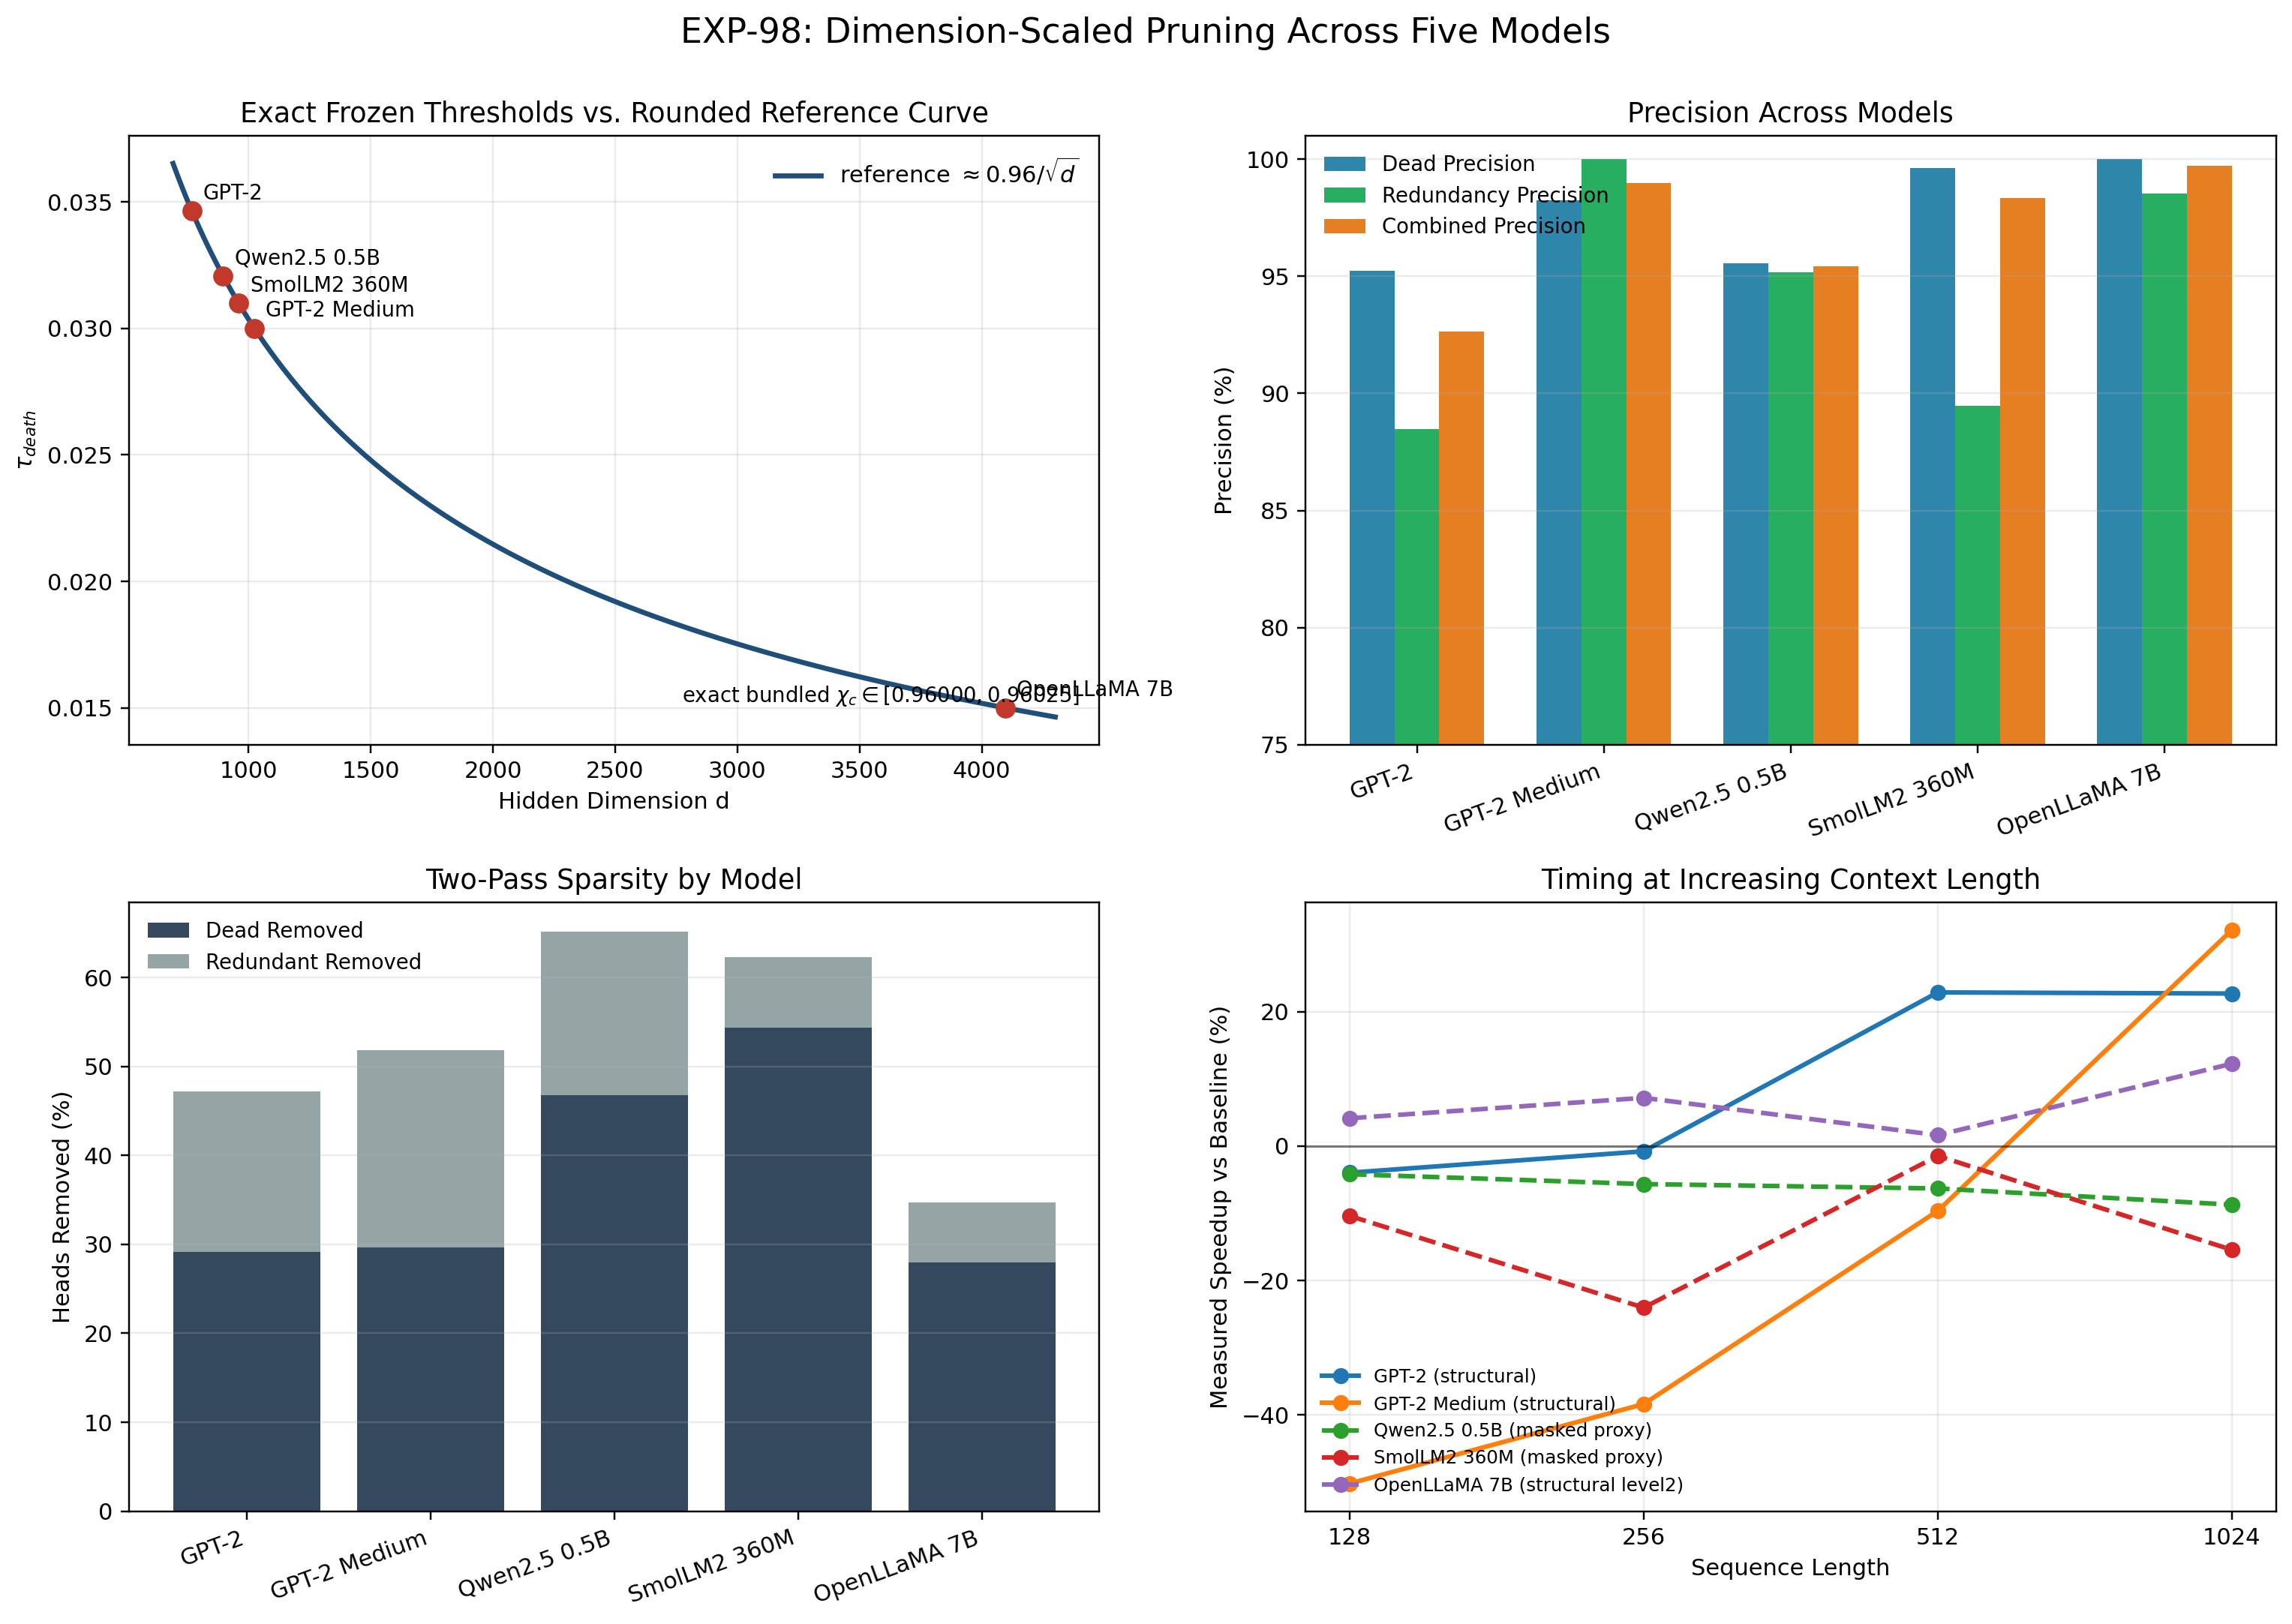
\includegraphics[width=\textwidth]{figures/exp98_five_model_summary.png}
\caption{\label{fig:five-model}
Five-model summary of the derived threshold curve, dead/redundancy precision,
resulting sparsity, and measured timing where structural compaction exists.}
\end{figure}

\subsection{Head-Level Threshold Evidence}

The threshold behavior is visible directly at head level once coupling is plotted in
normalized coordinates
\begin{equation}
z_h = \sqrt{d}\,\bar{c}_h,
\end{equation}
so that the bundled threshold boundary collapses to the narrow range
$0.96000 \le \chic \le 0.96025$.

Figure~\ref{fig:head-evidence} shows representative small-scale and LLaMA-scale
views. On GPT-2, $58/144$ heads fall below the threshold; $41$ of those are killed
and $13$ are retained only because boundary or bridge protection vetoes the death
decision. On OpenLLaMA 7B, $338/1024$ heads fall below threshold; $273$ of those
are killed and $34$ are protected. The GPT-2 dead-head false positives remain the
same two interior layer-5 heads. OpenLLaMA has no dead-head false positives on the
current pilot slice.

The normalized separation is also stable. For the five validated models, the dead
heads have normalized-coupling medians at or below zero, while the retained alive
heads have medians above $1.86$ and the redundant heads have medians above $2.72$.
The decision maps show the same structural pattern seen in the scalar statistics:
boundary protection is concentrated in the earliest layers, while dead heads
populate the interior of the network.

\begin{figure}[t]
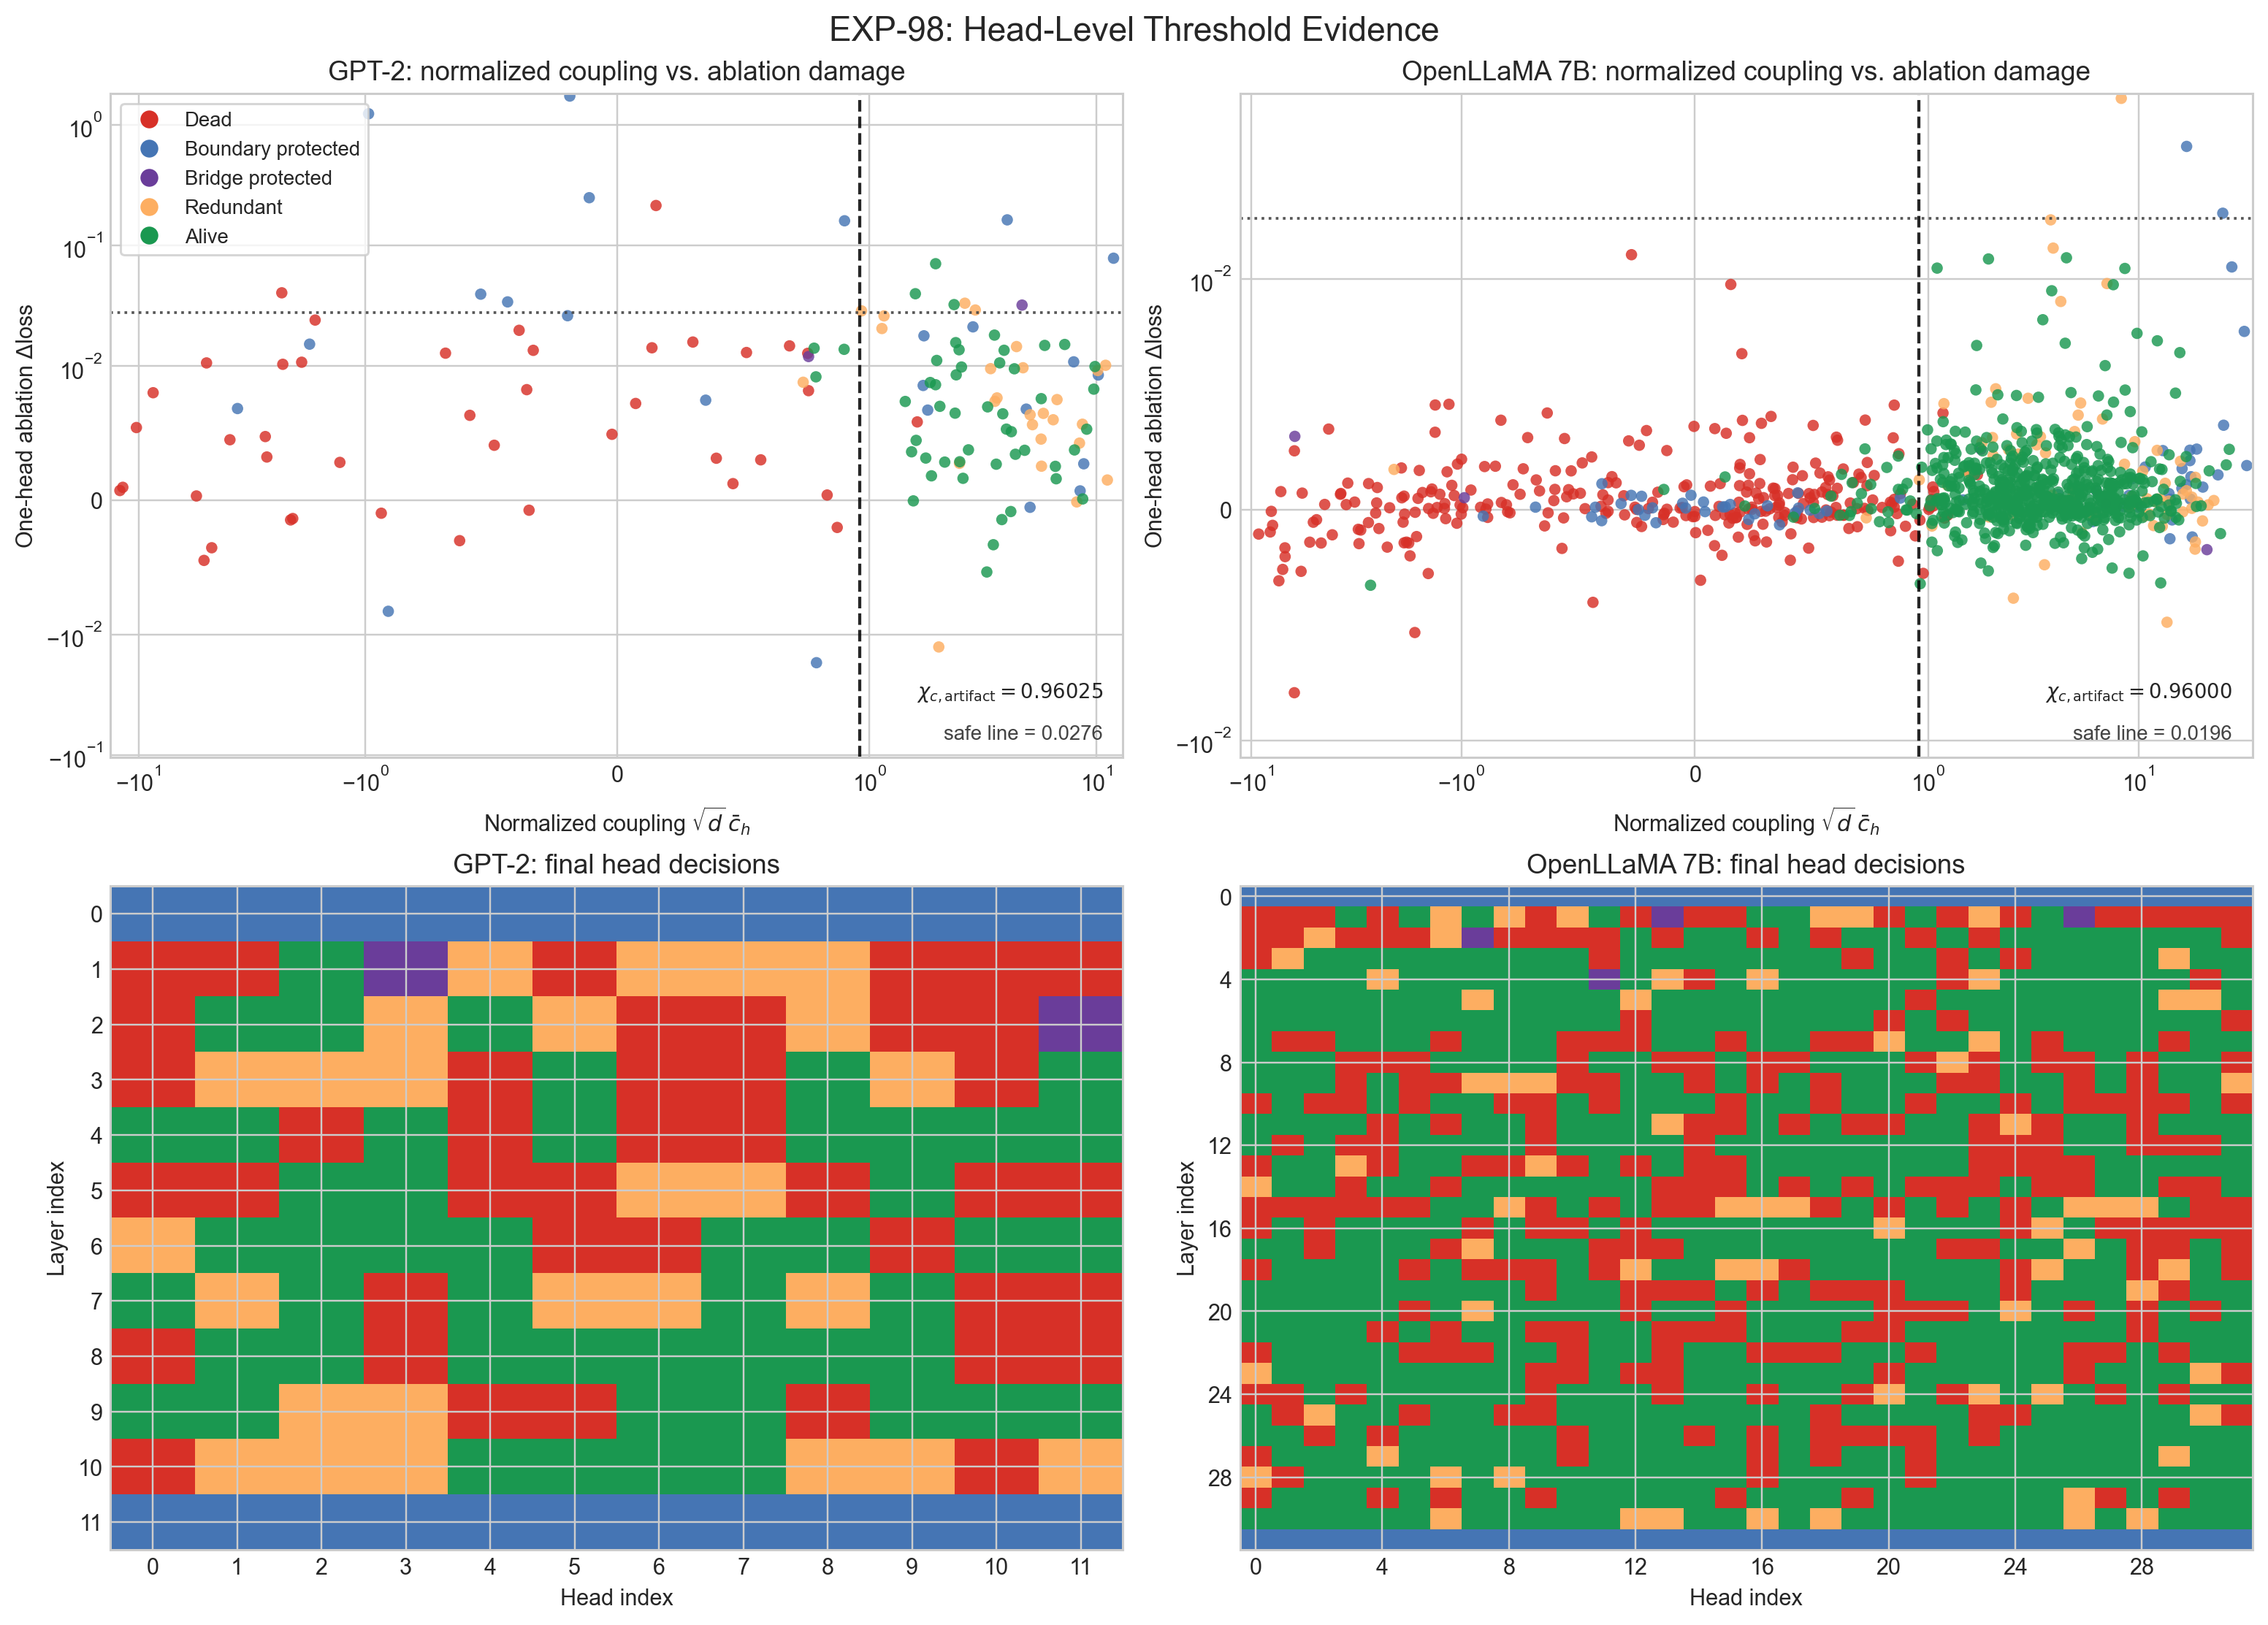
\includegraphics[width=\textwidth]{figures/exp98_head_threshold_evidence.png}
\caption{\label{fig:head-evidence}
Head-level threshold evidence. Top row: normalized coupling
$z_h=\sqrt{d}\,\bar{c}_h$ versus one-head ablation damage for GPT-2 and
OpenLLaMA 7B, with the exact artifact-specific normalized threshold drawn as a vertical dashed
line. Bottom row: categorical layer/head decision maps showing dead, protected,
redundant, and retained alive heads.}
\end{figure}

\subsection{Normalized Coupling Collapse}

Figure~\ref{fig:collapse} shows the same threshold in cross-model normalized
coordinates. Once $\bar{c}_h$ is rescaled by $\sqrt{d}$, the raw dimension
dependence is removed and the exact bundled thresholds collapse into a narrow band
near $z_h \approx 0.96$.

The left panel shows that the five bundled checkpoints occupy comparable normalized
ranges despite spanning hidden dimensions from $768$ through $4096$. The right panel
shows what happens to below-threshold heads after the protection rules are applied:
the majority become dead-head decisions, while most of the surviving minority is
explained by protection rather than by ordinary interior heads remaining alive
below threshold.

\begin{figure}[t]
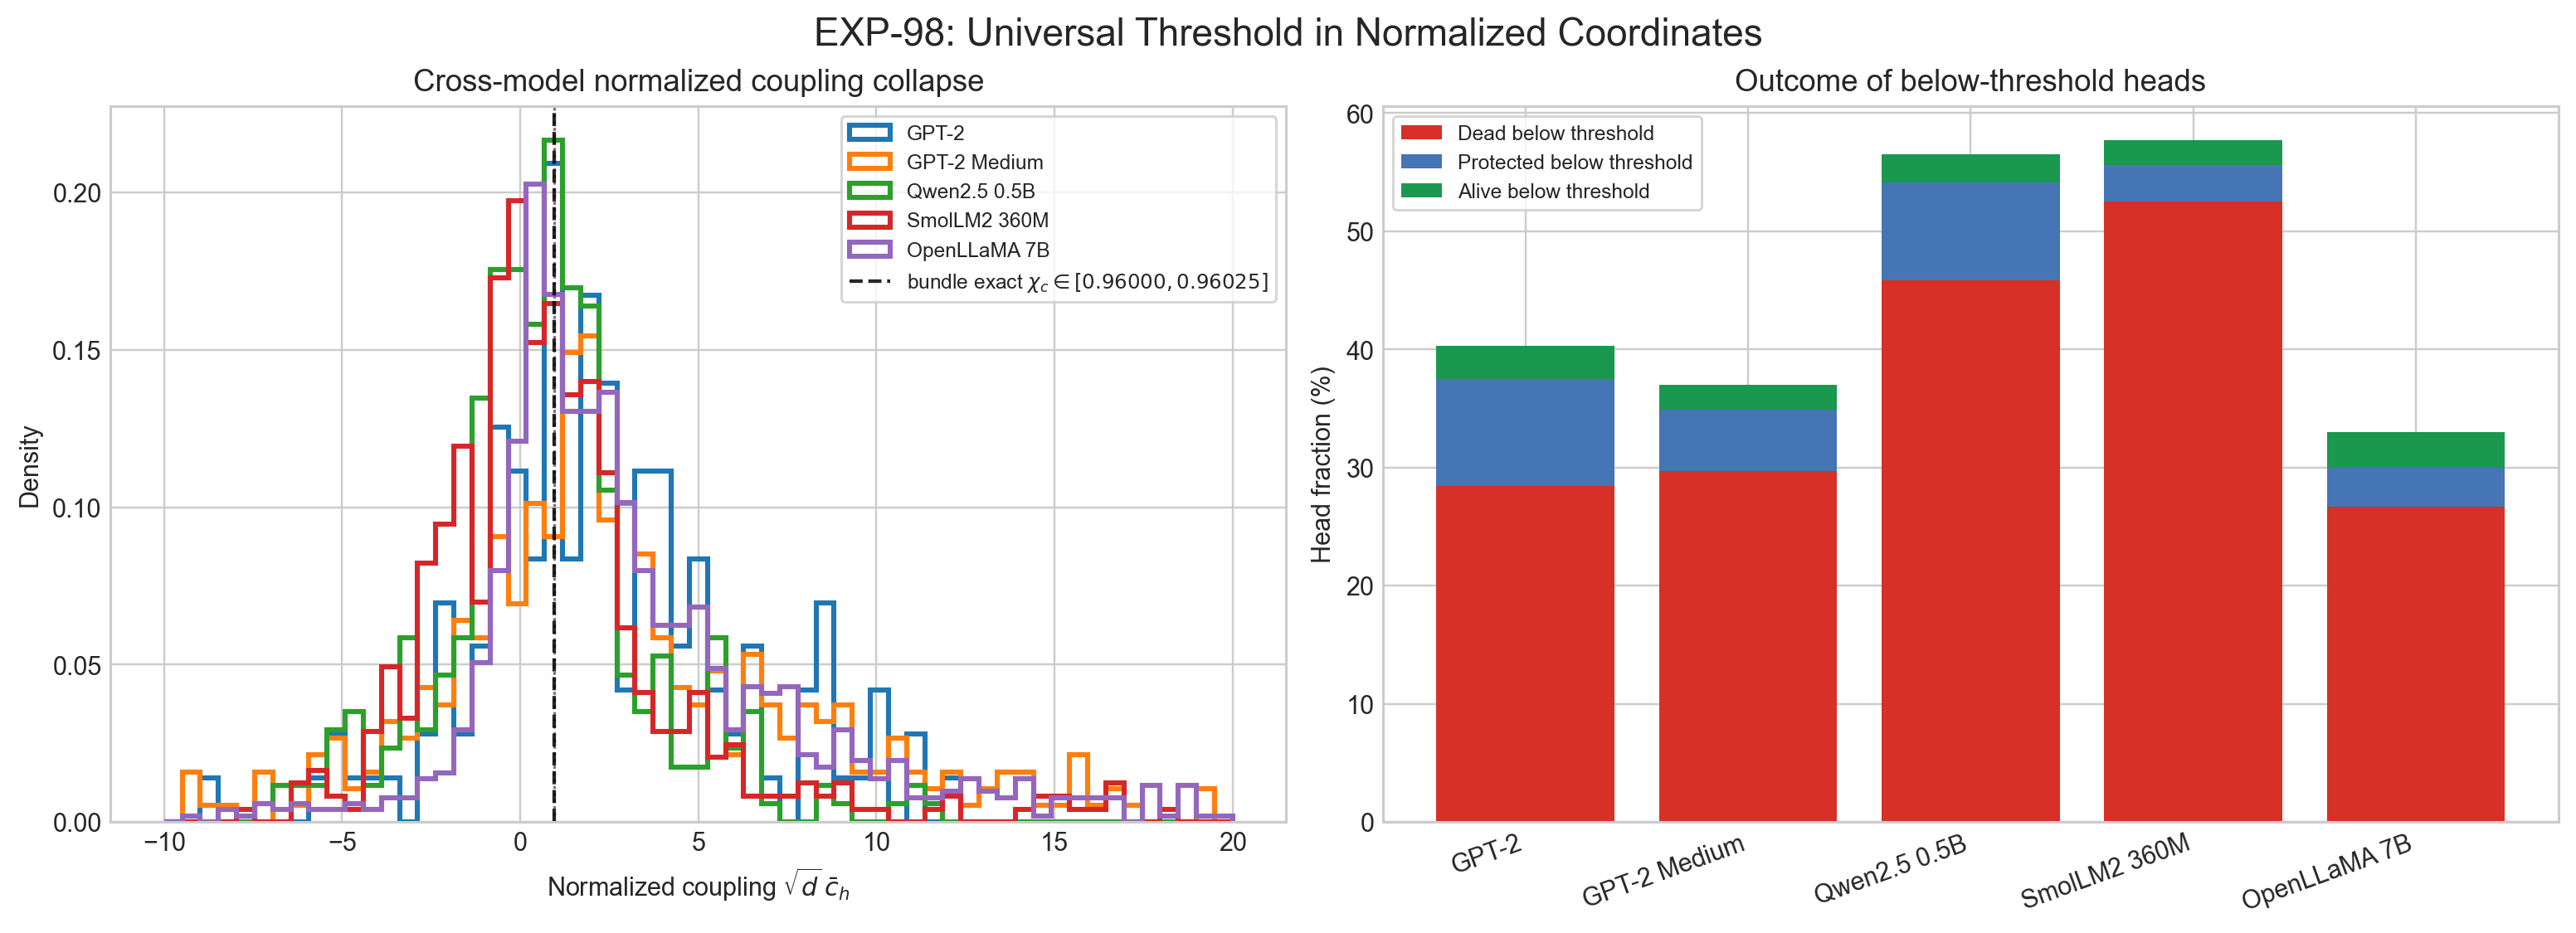
\includegraphics[width=\textwidth]{figures/exp98_normalized_coupling_collapse.png}
\caption{\label{fig:collapse}
Cross-model normalized coupling collapse. Left: all-head density in normalized
coordinates for the five completed models with the exact bundled thresholds
clustered at $\chic \in [0.96000, 0.96025]$. Right: model-wise breakdown of below-threshold heads into dead,
protected, and still-alive outcomes.}
\end{figure}

\subsection{Grouped-Query Level 2 Compaction}

SmolLM2 is the strongest grouped-query Level 2 target because its group size is only
$g=3$. The dead-head map induces:
\begin{equation}
44/160 = 27.5\%
\end{equation}
fully dead KV groups, with
\begin{equation}
132/480 = 27.5\%
\end{equation}
associated query heads removed. This yields:
\begin{itemize}
\item parameter count reduction: $361.8$M $\rightarrow 340.2$M ($-5.98\%$),
\item returned KV-cache reduction per token: $81{,}920 \rightarrow 59{,}392$
($-27.5\%$),
\item measured prefill speedup at sequence length $1024$: $+30.96\%$,
\item $\Delta$loss at sequence length $1024$: $+0.53206$.
\end{itemize}

The Qwen2 comparison is informative. With group size $g=7$, only $3/48$ KV groups
are fully dead. The group-size barrier suppresses pure Level 2 compaction
combinatorially. This is a structural reason to separate the threshold story from
the systems story.

\begin{figure}[t]
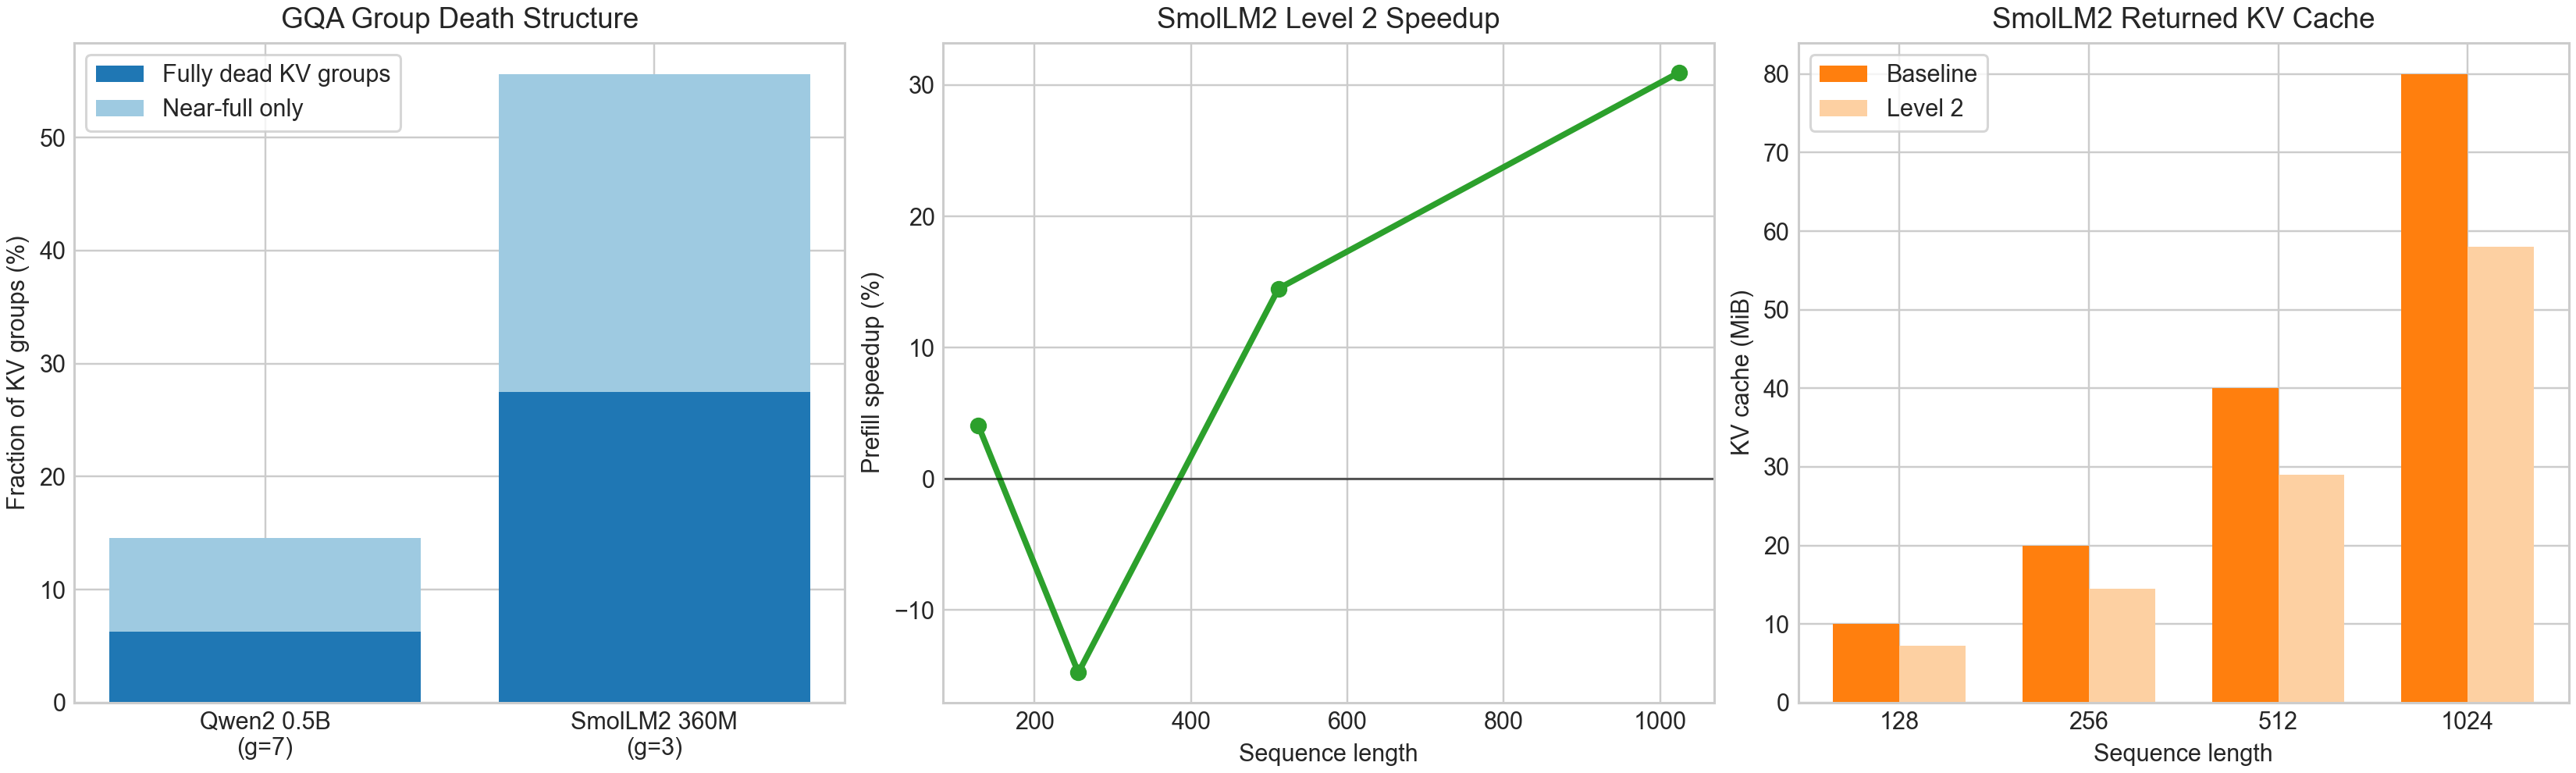
\includegraphics[width=\textwidth]{figures/exp98_gqa_level2_summary.png}
\caption{\label{fig:gqa}
Focused grouped-query result. SmolLM2's smaller group size makes full KV-group
death common enough for true Level 2 structural compaction; Qwen2's larger group
size does not.}
\end{figure}

\subsection{LLaMA-Scale Validation}

The OpenLLaMA 7B row is the key scaling test. At $d=4096$,
\begin{equation}
\taudeath(4096)=\frac{\chic}{\sqrt{4096}}\approx 0.015,
\end{equation}
and the dead pass produces:
\begin{itemize}
\item $286/1024$ dead heads,
\item $100.0\%$ dead-pass precision,
\item zero dead-head false positives on the current pilot slice.
\end{itemize}

Because OpenLLaMA 7B uses full multi-head attention ($g=1$), dead-head structural
compaction is already the Level 2 result. The measured structural outcome is:
\begin{itemize}
\item parameter reduction: $6.74$B $\rightarrow 6.14$B ($-8.90\%$),
\item KV cache reduction: $524{,}288 \rightarrow 377{,}856$ bytes per token
($-27.93\%$),
\item measured speedup at sequence length $1024$: $+12.25\%$,
\item $\Delta$loss at sequence length $1024$: $+1.15692$.
\end{itemize}

\subsection{Timing Matrix}

Table~\ref{tab:timing} summarizes the strongest sequence-length-$1024$ timing rows.

\begin{table}[t]
\caption{\label{tab:timing} Timing summary at sequence length $1024$.}
\begin{tabular}{lcccc}
\toprule
Model & Timing Mode & Variant & Speedup vs. Baseline & $\Delta$Loss \\
\midrule
GPT-2 & structural & dead+redundant & +22.69\% & +2.66609 \\
GPT-2 Medium & structural & dead+redundant & +32.14\% & +2.19939 \\
Qwen2.5 0.5B & masked proxy & dead+redundant & -8.72\% & +2.49661 \\
SmolLM2 360M & structural Level 2 & fully dead KV groups & +30.96\% & +0.53206 \\
OpenLLaMA 7B & structural dead-only & dead heads & +12.25\% & +1.15692 \\
\bottomrule
\end{tabular}
\end{table}

This cleanly separates the classification result from the runtime result:
\begin{itemize}
\item the formula already transfers across architectures,
\item runtime gains appear where true structural compaction exists,
\item large-group GQA still needs Level 3 rebalancing to unlock the same systems
payoff.
\end{itemize}

\section{Discussion}

The strongest result in this paper is not that coherence ``wins a ranking horse
race.'' It is that a threshold derived from oscillator criticality and
high-dimensional geometry identifies dead heads at high precision across five
architecturally distinct frozen decoders.

The dead-pass behavior is conservative by design. It finds the definitely dead
subset first. Many safe-but-kept heads are coherent yet redundant. That is why the
redundancy pass is treated as a distinct compaction mechanism rather than as a fix
to the death threshold itself.

The cumulative removal rows should therefore not be read as a lossless-pruning
claim. They are secondary measurements of what happens under particular removal
choices once the dead set has been identified.

The paper also clarifies a systems point. Transfer of the threshold and transfer of
runtime speed are not the same event. Qwen2 validates the classifier but still lacks
native grouped-query structural compaction. SmolLM2 validates both the classifier
and the first grouped-query structural pathway. OpenLLaMA 7B validates the large-$d$
transfer and a true structural speedup at LLaMA scale.

The same separation applies to cumulative removal quality. A head can satisfy the
dead-head identification law and still require compensation when many heads are
removed together, because multi-head deletion can perturb distributed basis
rotations across layers. That is why this paper validates the law with one-head
ablation precision rather than treating naive cumulative deletion as the theorem
target. Rotation-aware pruning operators, including SVD-based compensation
schemes, belong to follow-on engineering work.

Separate later CLR pipeline runs also continue to surface sizeable dead-head sets at
larger scale, e.g.\ $407$ dead heads ($26.5\%$) on REAP-25B MoE. We do not elevate
those rows into the main claim here because this publication bundle does not include
their matching per-head ablation ground truth.

Two natural follow-on papers are now separated from the present result:
\begin{enumerate}
\item a generalized BKT / vector-Kuramoto critical theory on $S^{d-1}$,
\item CLR-during-training, where dead heads and layers are removed online rather
than post hoc.
\end{enumerate}
Both are legitimate next steps, but neither is needed to support the present
publication claim.

\subsection{Independent Confirmation from Weight Compression}

An independent line of evidence strengthens the geometric picture.
Turney~\cite{Turney2026} recently conducted systematic A/B isolation of tensor
roles in transformer weight compression, discovering through brute-force ablation
that:
\begin{enumerate}
\item attention tensors tolerate WHT-rotated quantization well,
\item FFN write-back projections (\texttt{ffn\_down}) are quality-critical, and
\item boundary layers are disproportionately sensitive.
\end{enumerate}
These three findings were reached without reference to the CLR framework. Each
maps directly onto elements of the present paper:
\begin{itemize}
\item attention tolerance $\leftrightarrow$ inter-oscillator couplings operate near
the random-alignment scale, so moderate perturbation does not shift them across
the death boundary;
\item write-back sensitivity $\leftrightarrow$ the residual-stream output projection
is the coupling's \emph{write} channel into the shared state, where errors compound
layer-over-layer (same mechanism as K-error amplification through softmax in KV
cache compression);
\item boundary sensitivity $\leftrightarrow$ boundary layers act as driven lattice
boundary nodes under different dynamics from interior layers.
\end{itemize}

We applied the tensor-role insight to the CLR weight-quantization stage of our
compression pipeline (Stage~4b). Guided by the anatomy eligibility profile from
the \emph{same single forward pass} used for dead-head identification, attention
and FFN read projections receive 4-bit WHT-rotated quantization while FFN
write-back projections receive 6-bit protection. On Qwen3-8B
($d=4096$, 36 layers), this role-aware policy reduces the weight-quantization
quality cost from $\Delta\text{Loss}=+0.339$ (uniform 4-bit) to
$\Delta\text{Loss}=+0.038$ --- an \textbf{89\% reduction in quality loss} at
comparable effective bit rate (4.24 vs 3.69 bits). No additional calibration,
retraining, or Hessian computation is required; the anatomy profile already
contains the information needed.

This result is relevant to the present paper not as a pruning claim but as
\emph{convergent evidence}: the same coupled-oscillator geometry that identifies
dead heads also predicts which weight matrices tolerate compression and which
require protection. The tensor-role asymmetry discovered empirically by Turney is
a natural consequence of the distinction between inter-oscillator transport
channels (attention) and intra-oscillator modes (MLP) articulated in
Section~\ref{sec:mlp-modes}.

\section{Conclusion}

We presented a zero-parameter dead-head identification criterion for frozen
transformers:
\begin{equation}
\boxed{\taudeath(d)=\frac{\chic}{\sqrt{d}}}, \qquad \chic \approx 0.96.
\end{equation}
The threshold is derived, not fitted. Its observable is the mean cosine alignment
between a head's incoming write-back signal and the receiver's pre-head residual
state. Across GPT-2, GPT-2 Medium, Qwen2.5 0.5B, SmolLM2 360M, and OpenLLaMA 7B,
the dead-pass reaches $95.2\%$ through $100.0\%$ precision with no model-specific
recalibration when checked against individual head ablation. Structural compaction
results are secondary analyses and are not the core scientific claim of the paper.

The current paper therefore establishes a clean result: the coherence death
boundary transfers from lattice criticality into transformer head-death
identification through dimensional scaling. That is a meaningful publication
result even before the wider removal, generalized BKT, and training-time programs
are developed.

\appendix

\section{Reproducibility Package}

This publication folder is structured as a local package.

\begin{itemize}
\item \texttt{paper.tex}: formal manuscript source
\item \texttt{references.bib}: bibliography
\item \texttt{data/}: frozen JSON result artifacts
\item \texttt{figures/}: bundled figures
\item \texttt{scripts/98\_result\_plots.py}: regenerate the five-model summary
\item \texttt{scripts/98\_gqa\_level2\_plot.py}: regenerate the grouped-query figure
\item \texttt{scripts/98\_threshold\_evidence\_plots.py}: regenerate the head-level
threshold evidence and normalized-collapse figures
\item \texttt{scripts/98\_coherence\_pruning\_harness.py}: rerun the head-scan and
theory classification pass
\item \texttt{scripts/98\_verify\_threshold\_bundle.py}: verify the five bundled
transfer rows and write the machine-readable threshold summary
\item \texttt{scripts/98\_structural\_timing\_benchmark.py}: rerun structural timing
\item \texttt{scripts/98\_smollm2\_kv\_group\_compaction.py}: rerun grouped-query
Level 2 compaction
\end{itemize}

The included JSON artifacts are sufficient to rebuild the publication tables and
figures without rerunning the models. Full model reruns require access to the
relevant Hugging Face checkpoints and a calibration/evaluation corpus.

\bibliographystyle{apsrev4-2}
\bibliography{references}

\end{document}
